\section{Theorical Background}

\subsection{Tổng quan về công nghệ Bluetooth Low Energy (BLE)}

Bluetooth Low Energy (BLE) là một chuẩn truyền thông không dây trong băng tần ISM $2.4 GHz$, được thiết kế cho các ứng dụng IoT tiêu thụ năng lượng thấp. Chuẩn này sử dụng 40 kênh RF, trong đó có 3 kênh quảng bá (advertising) và 37 kênh dữ liệu, với tốc độ truyền danh định 1 Mbps và khoảng cách hoạt động khoảng 10–50 m tùy điều kiện.

Điểm khác biệt quan trọng giữa BLE và Bluetooth Classic là cơ chế tiết kiệm năng lượng. BLE chỉ phát gói tin ngắn trong quá trình quảng bá và duy trì trạng thái ngủ phần lớn thời gian, thay vì giữ kết nối liên tục. Điều này giúp thiết bị chạy bằng pin nhỏ có thể hoạt động trong nhiều tháng hoặc thậm chí nhiều năm.

Kiến trúc giao thức BLE gồm hai phần: Controller (lớp vật lý và liên kết, xử lý kết nối ở mức thấp) và Host (các giao thức cao hơn như ATT, GATT, GAP và quản lý bảo mật). Giao diện giữa hai phần được chuẩn hóa thông qua Host Controller Interface (HCI), cho phép linh hoạt trong phát triển phần cứng và firmware.

Trong hoạt động, thiết bị BLE có hai chế độ chính: advertising (phát gói tin để thông báo sự hiện diện, cho phép quét và thiết lập kết nối) và connection (trao đổi dữ liệu dựa trên profile GATT). Ngoài ra, thiết bị có thể ở trạng thái chờ (idle) hoặc deep-sleep, đảm bảo mức tiêu thụ dòng cực thấp.

\subsubsection{BLE protocol stack and working modes}

Controller (lowest layer of stack)

Host (upper layer protocol and runs the following services)

\subsubsection{BLE Beacons}

\subsubsection{BLE Development Basics}

\noindent\textbf{Bluetooth LE Protocol Architecture}

Trong Bluetooth protocol stack được chia làm 3 thành phần chính hoặc là các phần tử của hệ thống như sau: \textbf{application}, \textbf{host} and \textbf{controller}. Bên trong mỗi lớp đó có các lớp riêng biệt khác trong đó.

\begin{figure}[H]
	\centering
	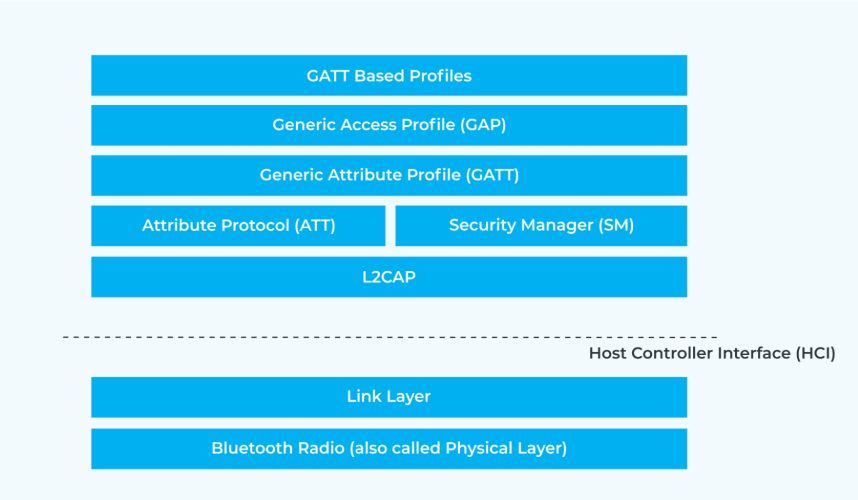
\includegraphics[width=.6 \linewidth]{./my-chapters/my-images/theoretical_background/BLE/BLE_protocol_stack.png}
	\caption{Bluetooth Radio in LE protocol stack.}
\end{figure}

\noindent\textbf{BLE Protocol Layers}

\begin{enumerate}[label=\arabic*)]
	\item The Physical Layer: được đề cập là một physical radio được sử dụng trong giao tiếp và cho việc modulation/demodulating dữ liệu. Nó được sử dụng trong các dải tần ISM ($2.4GHz$ spectrum).
	\item The Link Layer: là lớp giao tiếp với Physical Layer (Radio) và cung cấp cho các lớp cao hơn 
\end{enumerate}

\subsection{Kiến trúc và đặc điểm kỹ thuật của ESP32-C3}

ESP32-C3 là vi mạch SoC do Espressif phát triển, tích hợp nhân xử lý RISC-V 32-bit, xung nhịp 160 MHz và bộ nhớ SRAM 400 KB. Điểm mạnh quan trọng của C3 là hỗ trợ Bluetooth Low Energy 5.0 cùng Wi-Fi $2.4 GHz$, cho phép lựa chọn linh hoạt giữa truyền tải cự ly ngắn, tiêu thụ năng lượng thấp và kết nối Internet dung lượng lớn.

\begin{figure}[h]
	\centering
	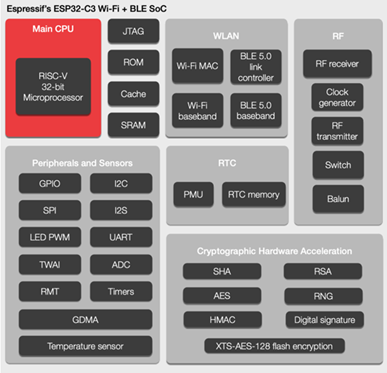
\includegraphics[width=.8\linewidth]{./my-chapters/my-images/theoretical_background/overview_block_diagram_for_esp32.png}
	\caption{Sơ đồ khối của ESP32-C3.}
\end{figure}

Trong bối cảnh đề tài, BLE 5.0 là thành phần trọng tâm, đảm bảo khả năng quảng bá, kết nối và truyền dữ liệu cảm biến với mức tiêu thụ năng lượng tối thiểu. ESP32-C3 cung cấp nhiều chế độ tiết kiệm năng lượng (light-sleep, deep-sleep), với dòng tiêu thụ trong deep-sleep chỉ vài µA, đáp ứng yêu cầu đo lường và tối ưu hóa năng lượng của hệ thống.

Bên cạnh đó, SoC này tích hợp ADC 12 bit, giao tiếp chuẩn SPI/I$^{2}$C/UART, cho phép kết nối trực tiếp với các cảm biến nhiệt độ, độ ẩm và ánh sáng. Nguồn cấp được quản lý thông qua LDO và mạch decoupling nhằm đảm bảo ổn định cho hoạt động của RF và khối xử lý.

Về phần mềm, ESP32-C3 được hỗ trợ bởi ESP-IDF, cung cấp sẵn stack BLE (GATT, GAP) và công cụ quản lý năng lượng. Điều này giúp nhóm tập trung phát triển firmware cho các chức năng chính: quảng bá dữ liệu, gửi thông báo định kỳ, xử lý ngắt từ GPIO wake-up, và đo lường độ trễ wake-up đến khi phát gói BLE đầu tiên.

\subsection{Quản lý năng lượng trong BLE node}

Đối với node BLE sử dụng ESP32-C3, quản lý năng lượng là yếu tố quan trọng quyết định đến khả năng vận hành trong thời gian dài. Đặc thù của hệ thống là việc truyền dữ liệu cảm biến chỉ diễn ra theo chu kỳ hoặc khi có sự kiện đánh thức, trong khi phần lớn thời gian thiết bị ở trạng thái chờ (idle).

Cách tiếp cận phổ biến nhất để giảm tiêu thụ năng lượng là tổ chức các chế độ hoạt động của vi điều khiển và bộ thu phát RF theo mô hình duty cycle. Trong hầu hết thời gian, hệ thống ở trạng thái deep-sleep với mức dòng chỉ vài microampere; khi có sự kiện kích hoạt từ bộ đếm thời gian hoặc ngắt ngoài (GPIO wake-up), vi điều khiển thức dậy, khởi tạo kết nối BLE, truyền gói dữ liệu cần thiết, sau đó quay trở lại chế độ ngủ. Độ trễ từ thời điểm wake-up đến khi phát gói BLE đầu tiên là một tham số quan trọng phản ánh khả năng đáp ứng của hệ thống, đồng thời ảnh hưởng đến thiết kế firmware và cấu hình phần cứng.

Ngoài việc lựa chọn chế độ ngủ phù hợp, thiết kế mạch nguồn cũng góp phần quyết định đến hiệu quả năng lượng. Việc sử dụng bộ ổn áp tuyến tính công suất thấp (LDO) cùng các tụ decoupling đúng cách giúp giảm nhiễu nguồn, đảm bảo hoạt động ổn định của RF trong khi vẫn duy trì mức tổn hao nhỏ. Đối với cảm biến tích hợp, việc lập chu trình lấy mẫu dữ liệu theo chu kỳ hợp lý cũng giúp cân bằng giữa mức tiêu thụ và độ chính xác của phép đo.

\subsection{Lý thuyết về Directional Coupler}

Directional coupler (bộ ghép định hướng) là một thành phần thụ động bốn cổng dùng để lấy mẫu (sample) năng lượng trên một đường truyền RF mà không làm nhiễu đáng kể tới đường truyền chính. Trong bối cảnh đề tài - giám sát và đo lường tín hiệu $2.4GHz$ của bộ phát BLE - dạng coupler thực thi chức năng cung cấp tín hiệu mẫu cho VNA, detector hoặc cho mạch Wake-Up Receiver, đồng thời cho phép đánh giá công suất truyền, phản sóng và phase. Phần tiếp theo trình bày những khái niệm lý thuyết cần thiết cho thiết kế microstrip coupled-line coupler, bao gồm nguyên lý hoạt động, tham số tán xạ và các đặc tính như coupling, isolation, insertion loss và phase mà nhóm tìm hiểu từ các tài liệu.

\begin{figure}[h]
	\centering
	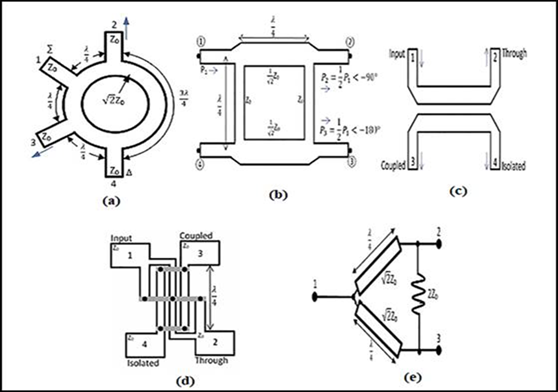
\includegraphics[width=.8\linewidth]{./my-chapters/my-images/theoretical_background/coupler_directional.png}
	\caption{Các cấu hình của Directional Coupler: a) Ring directional coupler; b) Branch-line directional coupler (c) Coupled-line directional coupler; (d) Lange directional coupler; (e) Wilkinson power divider.}
\end{figure}

\subsubsection{Nguyên lý vi dải và đường truyền song song (microstrip coupled-line)}

Microstrip coupled-line directional coupler là cấu trúc bao gồm hai dải vi dẫn song song đặt gần nhau trên cùng một lớp dieletric với mặt đất bên dưới; tương tác giữa hai dải tạo ra hiện tượng ghép điện từ (electromagnetic coupling). Khi một sóng điện từ chạy trên dải “chính” (through line), năng lượng sẽ được truyền một phần sang dải kề bên qua tương tác trường điện (even-mode) và trường từ (odd-mode). Ở tần số trung tâm, nếu chiều dài của đoạn ghép bằng một phần tư bước sóng dẫn ($l \approx \dfrac{\lambda_g}{4}$), các sóng even và odd kết hợp sao cho năng lượng được phân tách thành hai cổng: một cổng “through” (truyền chính) và một cổng “\textit{coupled}” (lấy mẫu) theo chiều định hướng mong muốn; cổng thứ tư (isolated) lý tưởng sẽ có năng lượng bằng 0.

\begin{figure}[H]
	\centering
	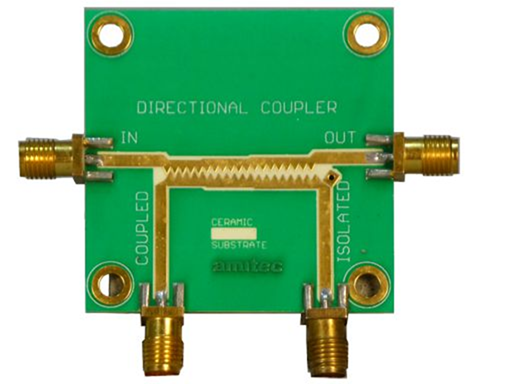
\includegraphics[width=.8\linewidth]{./my-chapters/my-images/theoretical_background/Cấu trúc của Directional Coupler.png}
	\caption{Cấu trúc của Directional Coupler.}
\end{figure}

Phân tích thường bắt đầu bằng các mode đối xứng (even) và phản đối xứng (odd). 
Mỗi mode có trở kháng đặc trưng khác nhau, gọi là $Z_{0e}$ (even-mode characteristic impedance) và $Z_{0o}$ (odd-mode characteristic impedance). 
Đối với mạch ghép cân bằng trên trở kháng hệ thống $Z_{0o}$, các quan hệ cơ bản là:
\[
Z_0=\sqrt{Z_{0e}Z_{0o}}
\]

Mối liên hệ giữa trở kháng mode và độ ghép (coupling coefficient) thường được định nghĩa bằng hệ số:
\[
k=\frac{Z_{0e}-Z_{0o}}{Z_{0e}+Z_{0o}}
\]
Giá trị $k$ xác định mức độ ghép điện áp giữa hai dải. Việc chọn chiều rộng dải, khoảng cách giữa hai dải và chiều dày/$\varepsilon_r$ của substrate ảnh hưởng trực tiếp tới $Z_{0e}$ và $Z_{0o}$, từ đó quyết định coupling mong muốn.

Trong thiết kế thực tế, để đạt coupling cố định tại tần số trung tâm người ta điều chỉnh các thông số hình học của coupled-line; để mở rộng băng thông, cần dùng nhiều đoạn ghép nối tiếp (multi-section) hoặc kỹ thuật bù dispersion.

\subsubsection{Tham số tán xạ (S-parameters)}

Bộ ghép định hướng được mô tả hiệu quả bằng ma trận tham số tán xạ $S$ bốn cổng. 
Với qui ước: 
\begin{itemize}[label=-]
	\item Cổng 1 là input,
	\item Cổng 2 là through,
	\item Cổng 3 là coupled,
	\item Cổng 4 là isolated,
\end{itemize}
ma trận $S$ của một coupler lý tưởng (mất mát bằng không, bắt khớp và cách ly hoàn hảo) có dạng:
\[
S=\begin{bmatrix}
	S_{11}&\cdots&S_{14}\\
	\vdots&\ddots&\vdots\\
	S_{41}&\cdots&S_{44}
\end{bmatrix}
\]

Trong đó, mỗi phần tử $S_{ij}$ (tất cả các cổng khác được ghép với tải chuẩn) được định nghĩa:
\[
S_{ij}=\frac{V_i^-}{V_j^+}
\]
với $i$ là ngõ vào, $j$ là ngõ ra; $V^-$: biên độ sóng phản xạ, $V^+$: biên độ sóng tới.

\subsubsection{Các hệ số đặc trưng}

\begin{itemize}[label=-]
	\item \textbf{Reflection Coefficients}: $S_{11}=S_{22}=S_{33}=S_{44}$ (khớp)
	\item \textbf{Transmission Coefficients}: $S_{12}, S_{34}, S_{43}, S_{21}=T$ (through coefficient)
	\item \textbf{Coupling Coefficients}: $S_{13}, S_{23}, S_{32}, S_{31}=C$ (coupled coefficient)
	\item \textbf{Isolation Coefficients}: $S_{14}, S_{24}, S_{42}, S_{41}=0$ (isolated port, lý tưởng là không có năng lượng)
\end{itemize}

Với mạch lý tưởng và mất mát bằng không, năng lượng bảo toàn đòi hỏi:
\[
|S_{21}|^2+|S_{31}|^2=1
\]

Trong thực tế, các thành phần tổn hao (conductor loss, dielectric loss, phasor mismatch) làm cho tổng trên nhỏ hơn 1; đồng thời $S_{41}\neq 0$ $\Rightarrow$ isolation hữu hạn.

Các đại lượng $S$ thường đo bằng VNA và được biểu diễn dưới dạng biên độ (dB) và phase (deg).

\subsubsection{Định nghĩa thực dụng}

\begin{itemize}[label=-]
	\item \textbf{Coupling Coefficients (Hệ số ghép)}:
	\[
	C=10\log{\left(\frac{P_{input}}{P_{coupled}}\right)}=-20\log_{10}\left|S_{13}\right| \ [\mathrm{dB}]
	\]
	
	\item \textbf{Directivity (Độ định hướng)}:
	\[
	D=10\log{\left(\frac{P_{coupled}}{P_{isolated}}\right)}=20\log_{10}\left|\frac{S_{13}}{S_{14}}\right| \ [\mathrm{dB}]
	\]
	
	\item \textbf{Isolation (Độ cách ly)}:
	\[
	I=10\log{\left(\frac{P_{input}}{P_{isolated}}\right)}=-20\log_{10}\left|S_{14}\right|=C+D \ [\mathrm{dB}]
	\]
	
	\item \textbf{Insertion Loss (Suy hao chèn)}:
	\[
	IL=10\log{\left(\frac{P_{input}}{P_{output}}\right)}=-20\log_{10}\left|S_{12}\right| \ [\mathrm{dB}]
	\]
\end{itemize}

Đo đồng thời biên độ và pha của $S_{21}$ và $S_{31}$ cho phép xác định coupler hoạt động như \textit{quadrature hybrid} hay coupler đơn thuần. Với coupler vi dải chuẩn $\ell=\lambda_g/4$, thường thu được quan hệ pha $\approx 90^\circ$ tại tần số trung tâm.

\subsubsection{Đặc tính thiết kế}

\begin{itemize}[label=-]
	\item \textbf{Coupling}: ví dụ $-10$ dB, $-20$ dB, xác định tỉ lệ năng lượng lấy mẫu.
	\[
	C=-20\log_{10}|k|,\quad k=\frac{Z_{0e}-Z_{0o}}{Z_{0e}+Z_{0o}}
	\]
	
	\item \textbf{Isolation}: cần $>20$–$30$ dB để tránh nhiễu ngược. Phụ thuộc vào độ đối xứng cấu trúc và sai số chế tạo.
	
	\item \textbf{Insertion Loss (IL)}: phản ánh tổn hao dẫn, dielectric, sai lệch trở kháng. IL càng nhỏ càng tốt.
	
	\item \textbf{Phase}: pha giữa tín hiệu through và coupled $\approx 90^\circ$ tại $f_0$, nhưng thay đổi theo tần số.
\end{itemize}

\subsubsection{Băng thông và đa đoạn}

Một cặp dải ghép đơn ($\lambda_g/4$) thường có băng thông hạn chế quanh tần số thiết kế. 
Để mở rộng băng thông và cải thiện độ phẳng về coupling, có thể dùng multi-section coupled line hoặc kỹ thuật bù.

